\documentclass {article}
\usepackage{ragged2e}
\usepackage{graphicx}
\usepackage{subcaption}
\usepackage[utf8]{inputenc}

\graphicspath{ {./images/} }

\title{IT Projekt}
\date{06.05.2019}
\author{Ivaylo Lenkov Ivanov}

\begin{document}

\begin{titlepage}
  \maketitle
  \tableofcontents
  \pagebreak
  \listoffigures
\end{titlepage}

\justify
\section{Einführung}
Für ein Hauptziel hat dieses Projekt eine virtuelle Umgebung zu bilden und in dieser Umwelt die grundlegende Physik zu simulieren. Die virtuelle Welt ähnelt ein Computerspiel.

\begin{figure}[h]
  \centering
  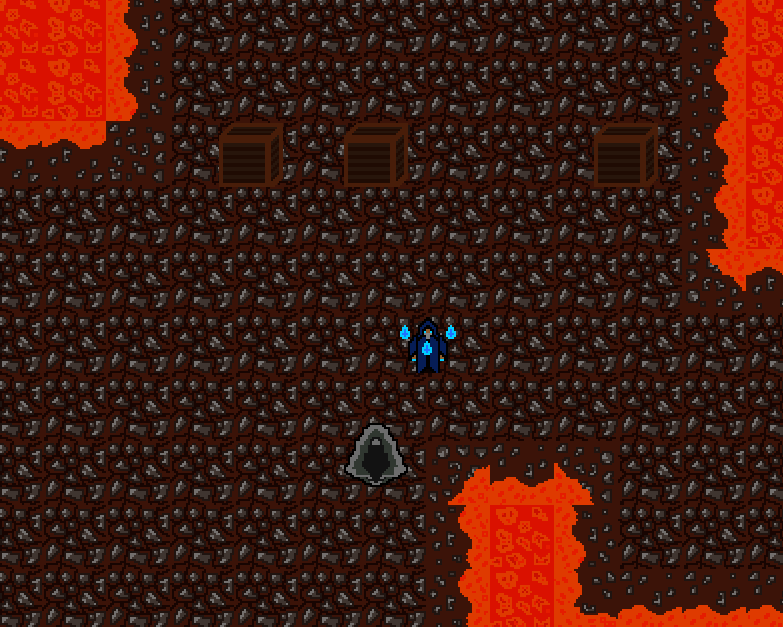
\includegraphics[scale=0.25]{VirtualEnvironment}
  \caption{Die virtuelle Umgebung}
  \label{fig:Umgebung}
\end{figure}

\justify
Der Benutzer steuert eine virtuelle Figur.

\begin{figure}[h]
  \captionsetup{justification=raggedright,singlelinecheck=false}
  
\includegraphics[scale=0.10]{MageCharacter}
  \caption{Avatar}
  \label{fig:Avatar}
\end{figure}

\justify
Der Avatar kann sich in dem Terrain bewegen und Eiszapfen in jeden Richtung feuern. Die Anfangsszene dem Spiel hat vier Spielobjekte --- drei Kasten und ein Stein.

\begin{figure}[h]
  \begin{subfigure}{0.5\textwidth}
    
\includegraphics[width=0.3\linewidth, height=2cm]{Box}
    \caption{Kasten}
    \label{fig:Kasten}
  \end{subfigure}
  \begin{subfigure}{0.5\textwidth}
    
\includegraphics[width=0.3\linewidth, height=2cm]{Stone}
    \caption{Stein}
    \label{fig:Stein}
  \end{subfigure}

  \caption{Spielobjekte}
  \label{fig:Spielobjekte}
\end{figure}

\justify
Mit den Kisten kann der Anwender interagieren. Das heißt, dass der Benutzer sie herumschubsen kann und auch auf sie Eiszapfen zu schießen. Das kann zu der Zerstörung diesen Kästen führen. Der Stein, der auch statisch Spielobjekt genannt wird, funktioniert wie eine Wand. Er ist unbeweglich und auch unverwüstlich.

In meisten virtuellen Produkten wird die Information durch irgendeiner Art von Animation präsentiert. Animation bedeutet sichtbare Bewegung. Das kann sehr wichtig sein, weil es ein Software viel mehr intuitiv macht. In den meisten Fällen die Systeme, die solche Lebhaftigkeit machen, sind Physik-Engines.

Implementieren die Physik in einem virtuellen Welt macht die Animationen, die Bewegungen und die Wechselwirkungen in diesem Welt immer flüssiger und realistischer und gibt immersives Erlebnis. Die Bilder sieht schöner und lebendiger aus. Diese Eigenschaften sind wichtig nicht nur in den Computerspielen, sonder auch in der virtual Reality, in der Software für visuelle Effekte und in den Anwendungen für Physik Simulation und für Animation.

Für dieses Projekt wird ein Spiel erstellt, wo die grundlegende physikalischer Gesetze gelten. In der virtuellen Welt gibt es eine Implementation von Beschleunigung, Kollisionserkennung, Kollisionsauflösung und elementare Teilchen.

Solche Umfeldern sind kompliziert und braucht viel Speicher. Man soll auch auf der Leistung der Software passen. Diese virtuelle Umgebung wird durch die Programmiersprache C++ erstellt. Auf diese Weise wird der Speicher sehr streng kontrolliert. Die Sprache erlaubt bessere Performance und macht die Anwendung auch portabel. Für den Computergrafik teil wird die Programmiere-Bibliothek ``SDL2'' benutzt. Die ``png'' Bilder werden mit der Hilfe von der Programmiere-Bibliothek ``SDL2-image'' geladen.

\newpage
\section{Überblick}
Wenn man das ganze Projekt betrachtet, kann man die Teile des Spiels bemerken --- Initialisierung, die Spiel-Schleife und Befreiung des Speichers.\\
Während der Initialisierung wird das Fenster, wo die virtuelle Welt dargestellt wird. Die Texturen werden geladen. Danach wird die initiale Szene des Spiels geschaffen.\\
Die nächste Phase ist die Spiel-Schleife. Das ist der Kern jedes Spiels --- ein endlose, aber überwachte Kreislauf. Hier werden die Dynamik und die Interaktivität der virtuellen Welt durchgeführt. Hier werden 4 Teile erkennt --- das Normieren von der Bildrate, ein Prüfung auf Ausfahrt, Aktualisieren der Spielszene und Vorbereiten den Objekten zum Rendern und
das Rendern der Änderungen. Damit die Bildfrequenz normieren können, wird die Zeit der Rahmen für ein Iteration der Spiel-Schleife gefunden. Wenn diese Uhrzeit ist kleiner als die festgelegte, dann wird die Bildrate nachdrücklich verzögert. Das ist wichtig, weil auf diese Weise die verschiedene Computer die gleich Bildfrequenz haben werden.\\
Der Kreis ist endlos, aber das bedeutet nicht, dass das Spiel kein Schluss hat. Drücken ein Taster wird als ein Event registriert. Auf diese Weise kommuniziert der Benutzer mit der virtuellen Umgebung. Solche Veranstaltungen werden gesammelt und werden bearbeitet. In diesem Projekt bricht das Drücken auf den Knopf ``ESC'' die Schleife.\\
Die Update-Phase \ldots


Dieses Projekt ist ein einfaches Computerspiel. Deswegen hat es die Struktur, die die übliche Spiele haben.
Der Kern jedes Spiels ist die Spiel-Schleife. Das ist eine endlose, aber überwachte Schleife. Da wird das Code geschrieben, das die Dynamik und die Interaktivität der virtuellen Welt enthielt. Normalerweise besteht der Loop aus verschiedene Teile. In diesem Fall hat die Schleife zwei Hauptbestandteile ---
\end{document}
